\documentclass{beamer}
\usepackage[utf8]{inputenc}
\usepackage{listings}
\usepackage{multicol}
\usetheme{Berlin}
\setbeamercolor{palette secondary}{use=seahorse}
\usecolortheme{seahorse}
\title[Developing with Docker]{Developing with Docker}
\author{\hspace{12pt}Robert “Anthony” Bittle\hspace{12pt}\\\hspace{12pt}robert.bittle@dominionenterprises.com\hspace{12pt}\\\hspace{12pt}github.com/guywithnose\hspace{12pt}}
\date{December 15, 2014}
\setbeamertemplate{itemize items}[circle]
\begin{document}
    \begin{frame}
        \titlepage
        Slides and demos at:\\
        \href{https://github.com/guywithnose/de-devcon-docker}{https://github.com/guywithnose/de-devcon-docker}\\
        \href{https://bitly.com/1vf4jcy}{https://bitly.com/1vf4jcy}
    \end{frame}

    % \section{Intro}
    % \begin{frame}{Who am I?}
    %     \begin{itemize}
    %         % Be quick, maybe cut this slide
    %         \item robert.bittle@dominionenterprises.com
    %         \item github.com/guywithnose
    %     \end{itemize}
    % \end{frame}
    \section{Docker}
    \subsection{What is Docker?}
    \begin{frame}{Similar to virtual machines...}
        % Similar to virtual machines, but without the overhead
        % Keep this high level use an image
        %
        % Why would a developer want a set up like this?
        % We upgrade system packages for one app without breaking all of our apps.
        \begin{figure}[htpb]
            \centering
            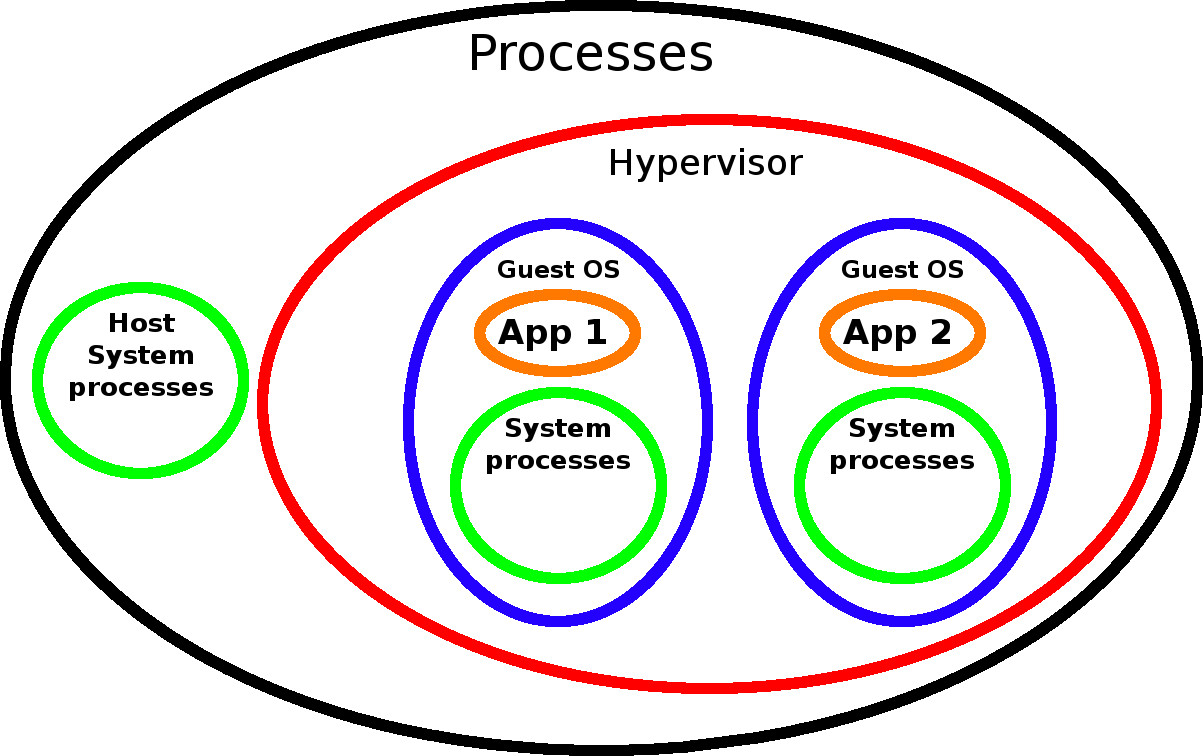
\includegraphics[width=0.8\linewidth]{VM.jpg}
        \end{figure}
    \end{frame}
    \begin{frame}{...only simpler}
        % Similar to virtual machines, but without the overhead
        % Keep this high level use an image
        \begin{figure}[htpb]
            \centering
            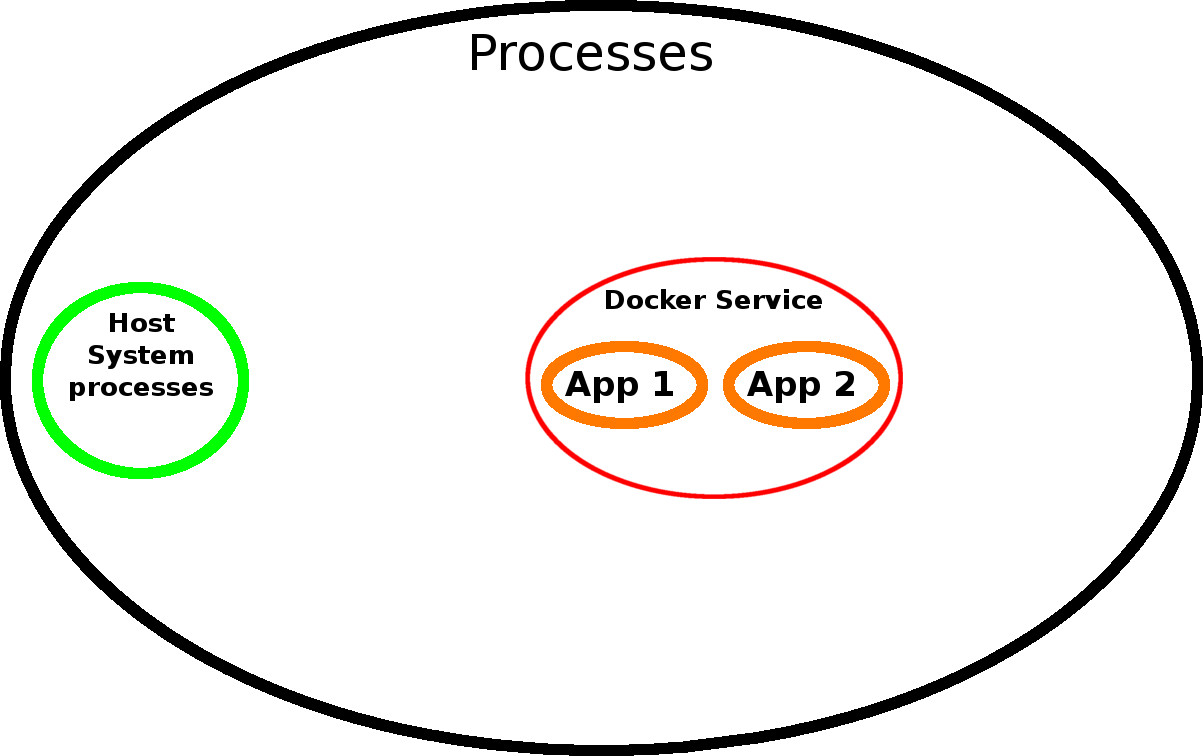
\includegraphics[width=0.8\linewidth]{Docker.jpg}
        \end{figure}
    \end{frame}
    % Basic comands
    \begin{frame}{Installation}
        \href{https://docs.docker.com/installation/}{https://docs.docker.com/installation/}
        \begin{itemize}
            \item Ubuntu, Red Hat, Debian, etc - Package manager
            \item OSX, Windows - Boot2Docker
        \end{itemize}
    \end{frame}
    \subsection{Working with images and containers}
    \begin{frame}{How to run a container}
        \alert<+>{docker run\alt<+->{ $\backslash$\\}{ nginx}}
        \alert<.>{\only<.->{$--$detach $\backslash$\\}}
        \alert<+>{\only<.->{$--$volume \$(pwd):/usr/share/nginx/html $\backslash$\\}}
        \alert<+>{\only<.->{$--$publish 80:80 $\backslash$\\}}
        \only<2->{nginx}\\
        \only<+>{\vspace{24pt}docker run $-$d $-$v \$(pwd):/usr/share/nginx/html $-$p 80:80 nginx}
    \end{frame}
    \begin{frame}{The Dockerfile}{Start from scratch}
        % The emphasis here is creating a reproducible environment
        \alert<+>{}
        \alert<+>{FROM ubuntu:14.10\\}
        \alert<+>{RUN apt-get update \&\& apt-get install -y php5-fpm\\}
        \alert<+>{CMD /usr/sbin/php5-fpm $--$nodaemonize\\}
    \end{frame}
    \begin{frame}{The Dockerfile}{Modify an existing image}
        \alert<+>{}
        FROM nginx\\
        \alert<+>{ADD nginx.conf /etc/nginx/conf.d/default.conf\\}
    \end{frame}
    \begin{frame}{The Dockerfile}{Reduce image size}
        FROM base/archlinux\\
        \only<+>{RUN curl http://\dots/solr-4.10.2.tgz $>$ solr-4.10.2.tgz\\RUN tar -xz solr-4.10.2.tgz\\RUN rm solr-4.10.2.tgz}
        \only<+>{RUN curl http://\dots/solr-4.10.2.tgz $>$ solr-4.10.2.tgz; $\backslash$\\tar -xz solr-4.10.2.tgz; $\backslash$\\rm solr-4.10.2.tgz}
    \only<+>{RUN curl http://\dots/solr-4.10.2.tgz $|$ tar -xz}
    \end{frame}
    \begin{frame}{Building the Dockerfile}
        docker build -t my-nginx .
    \end{frame}
    \begin{frame}{How to link images}
        % Ideally a docker container should run only one process This is not
        % strictly necessary, but it is the way Docker was designed to work If
        % your system requires more than one process (nginx, php-fpm, mongo,
        % etc...), you will need to link your containers together so they can
        % communicate.
        docker run $-$d \alert<2>{$--$name db} mysql\\
        docker run $-$d \alert<3>{$--$name phpfpm} $--$link \alert<2>{db}:mysql jprjr/php-fpm\\
        docker run $-$d $--$link \alert<3>{phpfpm}:phpfpm $-$p 80:80 my-nginx\\
    \end{frame}
    \begin{frame}{Common commands}
        \begin{itemize}
            \item docker run
            \item docker build
            \item docker kill
            \item docker rm
            \item docker exec
            \item docker cp
            \item docker diff
        \end{itemize}
    \end{frame}
    \section{Fig}
    \subsection{What is Fig?}
    \begin{frame}{Docker containers in groups}
        \begin{itemize}
            \item Fig manages groups of linked containers
            \item Very intuitive interface
            \item Allows you to spin up, shutdown, and remove a container and all its dependencies with a single command
        \end{itemize}
        % Useful for running containers in groups
        % This is essential for development environments
        % Keep this high level use the same image
        % Talk about this being incorporated into docker
    \end{frame}
    \begin{frame}{Installation}
        \href{http://www.fig.sh/install.html}{http://www.fig.sh/install.html}
        \begin{itemize}
            \item One line installer
            \item Compatible with boot2docker
        \end{itemize}
    \end{frame}
    \subsection{}
    \defverbatim[colored]\lstFigYmlNginx{
        \begin{lstlisting}
nginx:
    build: .
    volumes:
        - .:/usr/local/nginx/html
    links:
        - phpfpm:phpfpm
    ports:
        - 80:80
        \end{lstlisting}
    }
    \defverbatim[colored]\lstFigYmlPhpFpm{
        \begin{lstlisting}
phpfpm:
    image: jprjr/php-fpm
    volumes:
        - .:/srv/http
    links:
        - mysql:mysql
        \end{lstlisting}
    }
    \defverbatim[colored]\lstFigYmlMysql{
        \begin{lstlisting}
mysql:
    image: mysql
    environment:
        MYSQL_ROOT_PASSWORD: password
        \end{lstlisting}
    }
    \begin{frame}{How to build a group}
        docker run $-$d $--$name db mysql\\
        \lstFigYmlMysql
    \end{frame}
    \begin{frame}{How to build a group}
        docker run $-$d $--$name phpfpm $--$link db:mysql jprjr/php-fpm\\
        \lstFigYmlPhpFpm
    \end{frame}
    \begin{frame}{How to build a group}
        docker run $-$d $--$link phpfpm:phpfpm $-$p 80:80 my-nginx\\
        \lstFigYmlNginx
    \end{frame}
    \begin{frame}{Run, stop, rebuild}
        \begin{itemize}
            \item fig run
            \item fig up
            \item fig stop
            \item fig rm
            \item fig build
        \end{itemize}
    \end{frame}
    % Give a full demo of an nginx, php-fpm, mysql system
    \section{Appendix}
    \subsection{Docker in production}
    \begin{frame}{Modifications}
        \begin{itemize}
            \item $ADD$ code instead of mounting as a volume.
            \item Only use images that don't run as root.
            \item Use Docker Hub (or host your own)
        \end{itemize}
    \end{frame}
    \subsection{Alternatives}
    \begin{frame}{Kubernetes}
        \begin{itemize}
            \item Open Source
            \item Created by Google
            \item Similar to fig, but it is more suited to production
            \item Uses JSON configuration instead of YAML
        \end{itemize}
    \end{frame}
\end{document}
